\chapter{Unity}

Dans cette partie il s'agira finalement de parler du développement du module \texttt{Unity} utilisant la nouvelle plateforme mise en place dont il est question Chapitre~\ref{chap:protoHP}. Ce développement a été la parfaite occasion de tester et mettre à l'épreuve cette dernière et avoir un retour réel sur son utilisabilité.
Il sera discuté, dans un premier temps, des apports, mais aussi des enjeux, de la conception et de la cible du module où il sera rapidement aborder les difficultés rencontrés qu'elles soient liés à \texttt{Unity} ou à la nouvelle plate-forme. 
Dans un second temps, nous nous attarderons sur le développement d'une application avec ce module de façon a évaluer s'il réponds aux besoins et si il il y répond de façon efficace.
Pour finir, nous effectuerons une rapide comparaison entre la version actuelle et la version en développement des kit de développement (\texttt{Unity} et \texttt{Processing}) afin d'avoir une évaluation dans des conditions réelles d'utilisation et peut être des pistes d'améliorations de la version \texttt{Unity}.

\section{Module Unity}

L'objectif du module Unity est de permettre à ses utilisateurs d'exploiter la puissance de Nectar (logicielle et matérielle) de façon totalement intuitive afin qu'ils puissent développer des applications de réalité augmentée spatiale sans jamais avoir besoin de se soucier des problèmes liés à cette technologie comme la problématique de calibration du couple caméra projecteur par exemple.
Pour cela, il a fallut créer, dans Unity, les composants et les comportements cruciaux du système tels que les caméras, les caméras de profondeur, les projecteurs, les utilisateurs, la table, et bien d'autres. En plus de résoudre bon nombre de problèmes pour l'utilisateur, ces composants rendent possible la représentation du monde réel Figure~\ref{fig:unityrealworld}. Cette représentation est très importante car, dans le domaine de la réalité augmentée spatiale, où ce dit monde sert de base aux augmentations et, de ce fait, ne peut pas être négligé, en avoir une représentation virtuelle précise permet aux utilisateurs de concevoir leur application dans le même environnement que celui où elles seront projetées.

\begin{figure}[H]
\centering
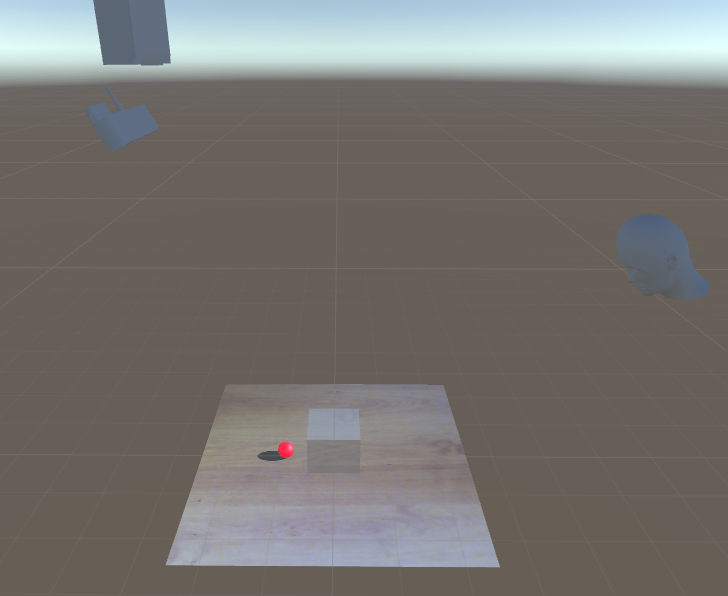
\includegraphics[width=0.7\linewidth]{images/unityscene}
\caption{Représentation du monde dans Unity - A droite, la tête de l'utilisateur, au centre la table, en haut a gauche le couple caméra projecteur.}
\label{fig:unityrealworld}
\end{figure}

Le module Unity possède actuellement deux types de composants:
\begin{itemize}
\item Les composants modélisant la partie matérielle qui correspondent aux différents dispositifs d'acquisitions (caméra projecteur).
\item Les composants modélisant la partie logiciel. Ils correspondent aux divers services de traitement fournis par Nectar.
\end{itemize}

Quelque soit son type les composants du module fonctionnent tous de la même façon. Tout d'abord chaque composant se connecte à Redis, c'est la base de données dans laquelle tous les services Nectar stock les informations qu'ils produisent. Une fois la connexion établie, le composant demande alors au serveur web Nectar l'état du service duquel il souhaite récupérer les données. Si le service est déjà exécuté, le composant peut alors commencer à récupérer et traiter les données que le service génère, sinon le composant demande au serveur de lancer le dit service. Le serveur web demande alors a Eye, le gestionnaire de processus, de démarrer le dit service et deux cas de figures peuvent se présenter. Soit le service démarre correctement et le composant peut commencer a en utiliser les données, soit le service ne peut pas être lancé. Dans ce cas le composant Unity cesse de fonctionner et fait remonter un avertissement à l'utilisateur.

% Chaque composant a son service (ou presque) et chaque composant peut demander a Nectar de lancer son service si il n'est pas lancé.

%il a dans un premier temps fallut créer un protocole permettant de récupérer dans Unity des informations envoyés par n'importe quel micro services.
Nous avons établies un protocole très simple

%Le développement s'est découpé selon deux axes principaux, a savoir récupérer et traiter les informations présente dans Redis pour les convertir et les utiliser dans Unity et proposer un ensemble de composants et de scripts 
% Importance du mode éditeur : controle a tout moment, état des services blabla -> très important pour l'utilisabilité du plugin.
%\subsection{Redis}
%Pour exploiter la nouvelle plateforme, le module devait avoir accès aux données produites par les micro services, centralisées dans Redis comme expliqué dans la section ~\ref{sec:nectararchi}.
%Les fondations du module Unity repose donc sur sa connexion  Redis ainsi qu'a la récupération des informations nécessaire.
% Connection a redis, reconstruction des images, protocol de transfert, affichage dans l'éditeur, execution en mode édition, intégration du control de nectar

% difficulté les reperes unity et processing pas la même came
%\section{Applications de démonstration}